\section{Ряды фурье}

\subsection{Определение ряда Фурье}

Далее, если не оговорено обратного, все интегралы будут интегралами Лебега.
\begin{definition}[Тригонометриеский ряд]
	Тригонометрическим рядом называется сумма вида:
	\begin{gather*}
		\frac{a_0}{2} + \sumlr{n = 1}{\infty} a_n \cos(nx) + b_n \sin(nx)
	\end{gather*}
	Частичные суммы тригонометрического ряда обозначаются $T_n(x)$
\end{definition}

Докажем несколько вспомогательных утверждений:
\begin{statement}
	Если $m \neq  n$ то
\begin{gather*}
	\intl{Q}\cos(nx)\sin(mx)dx = \intl{Q}\cos(nx)\cos(mx)dx = \intl{Q}\sin(nx)\sin(mx) = 0
\end{gather*}
\end{statement}
	
\begin{proof}
	\begin{enumerate}
		\item 
			\begin{gather*}
				\intl{Q}\cos(nx)\sin(mx)dx = 
				\frac{1}{2}\intl{Q}\left( \sin(x(n + m)) - \sin(x(n - m))\right) dx =\\
				\frac{1}{2}\left( -\frac{1}{n + m}\cos(x(n + m))\right)\Big|_{-\pi}^{\pi} -
				\frac{1}{2}\left( \frac{1}{n - m}\sin(x(n - m))\right)\Big|_{-\pi}^{\pi} = 0
			\end{gather*}
		\item
			\begin{gather*}
				\intl{Q}\cos(nx)\cos(mx)dx = 
				\frac{1}{2}\intl{Q}\left( \cos(x(n - m)) + \cos(x(n + m))\right) dx =\\
				\frac{1}{2}\left( \frac{1}{n - m}\sin(x(n - m))\right)\Big|_{-\pi}^{\pi} +
				\frac{1}{2}\left( \frac{1}{n + m}\sin(x(n + m))\right)\Big|_{-\pi}^{\pi} = 0
			\end{gather*}
		\item
			\begin{gather*}
				\intl{Q}\sin(nx)\sin(mx)dx = 
				\frac{1}{2}\intl{Q}\left( \cos(x(n - m)) - \cos(x(n + m))\right) dx =\\
				\frac{1}{2}\left( \frac{1}{n - m}\sin(x(n - m))\right)\Big|_{-\pi}^{\pi} -
				\frac{1}{2}\left( \frac{1}{n + m}\sin(x(n + m))\right)\Big|_{-\pi}^{\pi} = 0
			\end{gather*}		
	\end{enumerate}
\end{proof}

\begin{theorem}
	Пусть тригонометрический ряд сходится в пространстве $L_1$.
	Тогда для его коэффициентов выполнены формулы Эйлера-Фурье:
	\begin{gather*}
		a_0 = \frac{1}{\pi}\intl{Q}f(x)dx \\
		a_n = \frac{1}{\pi}\intl{Q}f(x)cos(nx)dx \\
		b_n = \frac{1}{\pi}\intl{Q}f(x)sin(nx)dx
	\end{gather*}
\end{theorem}

\begin{proof}
	Пусть $m, n \in \mathbb{N}, n > m$.
	Оценим следующий интеграл:
	\begin{gather*}
		\abs{\intl{Q}\left( f(x)\cos(mx) - T_n(x)\cos(mx)\right)dx} = \\
		\abs{\intl{Q}f(x)\cos(mx)dx - \intl{Q}\sumlr{k = 0}{n}A_k(x)\cos(mx)dx}\\
		\intl{Q}\sumlr{k = 0}{n}A_k(x)\cos(mx)dx = \sumlr{k = 0}{n}\intl{Q}A_k(x)\cos(mx) dx =\\
		\frac{a_0}{2}\intl{Q}\cos(mx)dx + \sumlr{k = 0}{n}\left(a_k\intl{Q}\cos(kx)\cos(mx)dx +
		b_k\intl{Q}\sin(kx)\cos(mx)dx\right) = a_m \intl{Q}\cos^2(mx)dx = \pi a_m \\
		\Rightarrow = \abs{a_m \pi - \intl{Q} f(x) \cos(mx) dx}
	\end{gather*}
	С другой стороны, нельзя не согласиться, что 
	\begin{gather*}
		\abs{\intl{Q}\left( f(x)\cos(mx) - T_n(x)\cos(mx)\right)dx} \leqslant \\
		\intl{Q}\abs{f(x) - T_n(x)} \abs{\cos(mx)} \leqslant \intl{Q}\abs{f(x) - T_n(x)} 
		\xrightarrow[n \rightarrow +\infty]{} 0 \Rightarrow \\
		\abs{a_m \pi - \intl{Q} f(x) \cos(mx) dx} = 0
	\end{gather*}
\end{proof}

\begin{corollary}
	Если тригонометрический ряд равномерно сходится на $Q$, 
	то его коэффициенты вычисляются по формулам ЭЙлера-Фурье.
\end{corollary}

\begin{definition}
	Пусть $f \in L_1$, тогда тригонометрический ряд с коэффициентами, 
	вычисленными по формулам Эйлера-Фурье, называется рядом Фурье функции $f$. 
\end{definition}

\begin{nb}
	Существуют сходящиеся тригонометрические ряды, которые не являются рядами Фурье своих сумм.
\end{nb}

\newpage

\subsection{Интеграл Дирихле}

Итак, для вывода интеграла Дирихле, рассмотрим частичную сумму ряда Фурье:

\begin{gather*}
	T_n(x) = \intl{Q}f(t)\frac{dt}{2\pi} + 
	\sumlr{k = 1}{n} \left( \intl{Q} f(t)\frac{1}{\pi}\cos(kt)dt\right) \cos(kx) + 
					 \left(	\intl{Q} f(t)\frac{1}{\pi}\sin(kt)dt\right) \sin(kx) = \\
	\intl{Q}f(t)\frac{1}{\pi} 
	\left(\frac{1}{2} + \sumlr{k = 1}{n} \cos(kt)\cos(kx) + \sin(kt)\sin(kx) \right)dt = \\
	\intl{Q}f(t) \frac{1}{\pi} \left( \frac{1}{2} + \sumlr{k = 1}{n} \cos(k(t - x))\right)dt
\end{gather*}

\begin{definition}[Ядро Дирихле]
	\begin{gather*}
		D_n(t) \defeq \frac{1}{\pi} \left( \frac{1}{2} + \sumlr{k = 1}{n} \cos(kt)\right)
	\end{gather*}
\end{definition}

\begin{definition}[Интеграл Дирихле]
	Частичные суммы тригонометрического ряда в следующем виде называют интегралом Дирихле.
	\begin{gather*}
		T_n(x) = \intl{Q} f(t) D_n(x - t)dt
	\end{gather*}
\end{definition}

Так как $D_n(t) = D_n(-t) \Rightarrow 
T_n(x) = \intlr{0}{\pi} \left( f(x + t ) + f(x -t )\right)D_n(t)dt$ 
(Здесь мы пользуемся периодичностью $f$).

\begin{statement}
	\begin{gather*}
		D_n(t) = \frac{1}{2\pi}\frac{\sin((n + \frac{1}{2})t)}{\sin\frac{t}{2}}
	\end{gather*}
\end{statement}

\begin{proof}
	\begin{gather*}
		\sin\frac{t}{2}D_n(t) =
		\frac{1}{\pi} \left( \frac{1}{2}\sin\frac{t}{2} +
		\sumlr{k = 1}{n} \cos(kt)\sin\frac{t}{2}\right) = 
		\frac{1}{\pi} \left( \frac{1}{2}\sin\frac{t}{2}+ 
		\frac{1}{2}\sumlr{k = 1}{n} \sin(k + \frac{1}{2})t - \sin(k - \frac{1}{2})t\right) = \\
		\frac{1}{2\pi}\sin(n + \frac{1}{2})t
	\end{gather*}
\end{proof}

Из формулы ясно, что $D_n(t)$ меняет знак с увеличением  $n$ все чаще, и можно показать, что 
\begin{gather*}
	\intl{Q} \abs{D_n(t) dt} \sim \ln n
\end{gather*}

Это заметно усложняет изучение рядов фурье в отдельных точках.

Очевидно, $\intl{Q}D_n(t) dt = 1$, следовательно $f(x) = \intlr{0}{\pi} 2 f(x) D_n(t) dt$.
Тогда можно записать разность в следующем виде:
\begin{gather*}
	T_n(x) - f(x) = \intlr{0}{\pi} \left(f(x + t) + f(x - t) - 2 f(x)\right)D_n(t) dt
\end{gather*}

Обозначим
$\phi(x, t) \defeq \left(f(x + t) + f(x - t) - 2 f(x)\right)$

И тогда получится 
\begin{gather*}
	T_n(x) - f(x) = \intlr{0}{\pi} \phi(x, t) D_n(t) dt
\end{gather*}

Эта формула нам пригодится в дальнейшем.

\subsection{Лемма Римана-Лебега}

\begin{lemma}[Лемма Римана-Лебега]
	Пусть $f \in L_1$ - суммируема на $\mathbb{R}$. Тогда
	\begin{gather*}
		\intl{\mathbb{R}} f(x) \cos nx dx \xrightarrow[n \rightarrow +\infty]{} 0\\
		\intl{\mathbb{R}}f(x) \sin nx dx  \xrightarrow[n \rightarrow +\infty]{} 0
	\end{gather*}
\end{lemma}

\begin{corollary}
	Если $f \in L_1$, то $a_n, b_n \xrightarrow[n \rightarrow +\infty]{} 0$
\end{corollary}

\begin{proof}[Доказательство следствия]
	$\pi a_n(f) = \intl{Q} f(x)\cos nx dx$. Пусть
	\begin{gather*}
		g(x) = 
		\left\{\begin{matrix}
			f(x), & x\in Q\\
			0,   & \text{otherwise} 
		\end{matrix}\right.
	\end{gather*}
	Тогда $\intl{\mathbb{R}}\abs{g} = \intl{Q}\abs{f}<+\infty$. 
	Следовательно $g$ - суммируема на числовой оси. 
	Следовательно $\intl{\mathbb{R}}g \cos nx dx \xrightarrow[n \rightarrow +\infty]{}0$.
	Но $\intl{\mathbb{R}}g \cos nx dx = \intl{Q}f \cos nx dx = \pi a_n(f)$
\end{proof}

\begin{proof}[Доказательство Леммы]
	Для доказательства леммы воспользуемся теоремой Лузина. 
	Для забывчивых, напомним ее формулировку:
	\begin{theorem}[Теорема Лузина]
		Пусть $E \subset \mathbb{R}^n$, $f \text{ - измерима на } E$. Тогда 
		$\feps > 0 \exists\phi \text{ - непрерывная на } \mathbb{R}^n : 
		\mu(f \neq \phi) < \Epsilon$. И если $\abs{f(x)}\leqslant M$ на $E$, то 
		$\abs{\phi(x)} \leqslant M$ на $\mathbb{R}$.
	\end{theorem}
	Доказательство будем вести в несколько этапов.
	Сначала покажем, что для любой функции суммируемой на оси и $\feps > 0 \exists g$ - 
	непрерывная и ограниченная на оси, такая, что $\normpp{f - g}{1} \leqslant \Epsilon$. 

	Так как $\intl{\mathbb{R}}f < +\infty$, то, по свойствам интеграла, 
	$\feps > 0$ существует множество конечной меры $E$ на котором функция $f$ - ограничена, 
	и при этом
	$\intl{\mathbb{R}\setminus E}\abs{f} < \Epsilon$. Теперь, по теореме Лузина,
	подберем $g$ - непрерывную на $\mathbb{R}$ и ограниченую $M$ функцию.
	Определим 
	\begin{gather*}
		\hat{f}(x) = 
		\left\{\begin{matrix}
			f(x), & x \in E \\
			0, & \text{otherwise}
		\end{matrix}\right.
	\end{gather*}
	Тогда $\intl{\mathbb{R}} \abs{f - \hat{f}} dx = \intl{\mathbb{R}\setminus E} \abs{f} < \Epsilon$.
	Ясно, что, так как $f$ - ограничена на $E$, 
	то $\hat{f}$ - ограничена той же константой на всей оси.
	По теореме Лузина, $\lambda\mathbb{R}(f \neq g) < \frac{\Epsilon}{M}$; 
	обозначим $E' = \mathbb{R}(f \neq g)$.
	Теперь 
	\begin{gather*}
		\intl{\mathbb{R}}\abs{f - g} \leqslant \intl{\mathbb{R}}\abs{f - \hat{f}} +
		\intl{\mathbb{R}}\abs{\hat{f} - g}
	\end{gather*}
	\begin{enumerate}
		\item $\intl{\mathbb{R}} \abs{\hat{f} - f} < \Epsilon$
		\item $\intl{\mathbb{R}} \abs{\hat{f} - g} = \intl{E'} \abs{\hat{f} - g} \leqslant 
			2M \lambda E' = 2M \frac{\Epsilon}{M} = 2\Epsilon$
	\end{enumerate}
	\begin{gather*}
		\intl{\mathbb{R}} \abs{f - g} \leqslant 3\Epsilon
	\end{gather*}
	
	Терперь проверим лемму Римана-Лебега для $g$.
	Мера Лебега $\sigma$-конечна, из этого следует, что(это надо чекнуть \todo)
	в качестве $E$ можно брать конечный промежуток.
	$E = \left< a, b\right>$. Рассмотрим $\abs{\intl{\mathbb{R}} g(x) \cos nx dx} = 
	\intl{\mathbb{R} \setminus \left< a, b \right>} \abs{g(x) \cos nx }dx +
	\intl{\left<a, b \right>} \abs{g(x) \cos nx} dx$
	\begin{enumerate}
		\item $\intl{\mathbb{R} \setminus \left< a, b \right>} \abs{g(x) \cos nx }dx \leqslant 
			\intl{\mathbb{R} \setminus \left< a, b \right>} \abs{g(x)}dx  < \Epsilon$
		\item $\abs{\intl{\left<a, b \right>} g(x) \cos nx} dx = 
			\abs{\intlr{a}{b} g(x)d\left( \frac{1}{n}\sin nx \right)} \leqslant 
			\abs{g(x)\frac{1}{n}\sin nx\Big|_{a}^{b}} + 
			\abs{\frac{1}{n}\intlr{a}{b}\sin nx d\left( g(x)\right)}$
			\begin{enumerate}
				\item $g(x)\frac{1}{n}\sin nx\Big|_{a}^{b} \xrightarrow[n \rightarrow +\infty]{} 0$
				\item $\abs{\frac{1}{n}\intlr{a}{b}\sin nx d\left( g(x)\right)} \leqslant 
					\frac{1}{n} \intlr{a}{b} \abs{d(g(x))} \xrightarrow[n \rightarrow +\infty]{} 0$ 
			\end{enumerate}
	\end{enumerate}

	Теперь докажем лемму для $f$. $\abs{\intl{\mathbb{R}}f(x) \cos nx} \leqslant 
	\intl{\mathbb{R}}\abs{f - g}\abs{\cos nx} dx + \abs{\intl{\mathbb{R}} g(x)\cos nx dx}$.
	\begin{enumerate}
		\item $\intl{\mathbb{R}}\abs{f - g}\abs{\cos nx} dx \leqslant
			\intl{\mathbb{R}}\abs{f - g} dx < \Epsilon $
		\item $\abs{\intl{\mathbb{R}} g(x)\cos nx dx} \xrightarrow[n \rightarrow +\infty]{} 0$
	\end{enumerate}
	Для синуса аналогично.
\end{proof}

Из этой леммы вытекает важное свойство рядов Фурье, описаное в следующем параграфе.

\subsection{Принцип локализации Римана}

\begin{theorem}[Принцип локализации Римана]
	Пусть $g, f$ - суммируемы и $2\pi$ - периодичны, а так же в $\delta$-окрестности некоторой точки $x$
	их значения совпадают, тогда 
	\begin{gather*}
		\lim\limits_{n\rightarrow +\infty} S_n(f, x) - S_n(g, x) = 0
	\end{gather*}
\end{theorem}

\begin{proof}
	Для простоты, представим, что у нас $x = 0$. Тогда
	\begin{gather*}
		S_n(f, x) - S_n(g, x) = \intl{Q} \left(f(x + t) - g(x + t) \right) D_n(t) dt = \\
		\intlr{-\pi}{-\delta} \left(f(x + t) - g(x + t) \right) D_n(t) dt +
		\intlr{\delta}{\pi} \left(f(x + t) - g(x + t) \right) D_n(t) dt
	\end{gather*}
	Будем оценивать такой интеграл(для остальных аналогично):
	\begin{gather*}
		\intlr{\delta}{\pi}f(x + t) \frac{1}{2\pi}
		\frac{\sin \left(n + \frac{1}{2} \right) t}{\sin \frac{t}{2}}
	\end{gather*}
	Перепишем $D_n(t)$:
	\begin{gather*}
		\frac{\sin \left(n + \frac{1}{2} \right) t}{\sin \frac{t}{2}} =
		\frac{\sin nt \cos \frac{t}{2} + \cos nt \sin \frac{t}{2}}{\sin\frac{t}{2}} = 
		\sin nt\ctg\frac{t}{2} + \cos nt
	\end{gather*}
	Далее, заметим важную вещь, которая заставляет все работать:
	При $\frac{\delta}{2} \leqslant \frac{t}{2} \leqslant \frac{\pi}{2}$, $\ctg\frac{t}{2}$ - ограничен.
	Получается, что $f(x + t)\ctg \frac{t}{2}$ и $f(x + t)$ - обе суммируемые функции, 
	а значит, для них выполнены условия леммы Римана-Лебега, отсюда получаем требуемое.
\end{proof}

\subsection{Теорема Фейера}

\begin{definition}[Сумма Фейера]
	\begin{gather*}
		\sigma_n(f, x) \defeq \frac{1}{n + 1} \sumlr{k = 0}{n} S_k(f, x)
	\end{gather*}
\end{definition}

Получим ее форму через интеграл:

\begin{gather*}
	\sigma_n(f, x) = \frac{1}{n + 1} \sumlr{k = 0}{n} \intl{Q} f(x + t)D_n(t) dt = 
	\intl{Q} f(x + t) \left( \frac{1}{n + 1} \sumlr{k = 0}{n} D_k(t)dt\right)
\end{gather*}

\begin{definition}[Ядро Фейера]
	\begin{gather*}
		\Phi_n(t) \defeq  \frac{1}{n + 1} \sumlr{k = 0}{n} D_k(t)dt
	\end{gather*}
\end{definition}

\begin{definition}[Интеграл Фейера]
	\begin{gather*}
		\sigma_n(f, x) = \intl{Q} f(x + t)\Phi_n(t)dt
	\end{gather*}
\end{definition}

\begin{statement}
	\begin{gather*}
		\Phi_n(t) = 
		\frac{1}{2\pi(n + 1)}\left(\frac{\sin(\frac{n + 1}{2} t)}{\sin\frac{t}{2}} \right)^2
	\end{gather*}
\end{statement}

\begin{theorem}[Теорема Фейера]
	Пусть $f \in L_1$, $f$  - периодична с периодом $T$. 
	Пусть $\\ \phi_x(t) = f(x + t) + f(x - t) - 2S$.
	Пусть $\frac{1}{t} \intlr{0}{t}\abs{\phi_x(t)} \xrightarrow[t \rightarrow 0]{} 0$.
	Тогда 
	\begin{gather*}
		\sigma_n(f, x) \xrightarrow[n \rightarrow 0]{} S
	\end{gather*}
\end{theorem}

\begin{proof}
	Пусть $h_n = \frac{1}{n + 1}$. $\sigma_n(f, x) - S 
	= \intlr{0}{\pi} \phi_x(t)\Phi(t)dt$.
	Разобьем интеграл на два $\intlr{0}{\pi} = \intlr{0}{h_n} + \intlr{h_n}{\pi}$.
	\begin{gather*}
		\abs{\sigma_n(f, x) - s} \leqslant \intlr{0}{h_n} \abs{\phi_x(t)} \Phi(t)dt +
		\intlr{h_n}{\pi} \abs{\phi_x(t)} \Phi(t)dt
	\end{gather*}
	Заметим, что $\abs{\sin nt} \leqslant n \abs{\sin t} \Rightarrow \Phi_n(t) \leqslant 
	\frac{1}{2\pi h_n}$, следовательно $\intlr{0}{h_n} \abs{\phi_x(t)} \Phi(t)dt \leqslant
	\frac{1}{2\pi} \frac{1}{h_n} \intlr{0}{h_n} \abs{\phi_x(t)}dt 
	\xrightarrow[n \rightarrow 0]{} 0$  
	Рассмотрим $\intlr{h_n}{\pi}\abs{\phi_x(t)}\Phi_n(t)dt$.
	При $t \in \left[ 0, \frac{\pi}{2}\right], \sin t \geqslant \frac{2}{\pi}t$, 
	тогда $\Phi_n(t) \leqslant \frac{h_n}{2\pi} \frac{1}{\sin^2\frac{t}{2}} \leqslant
	\frac{h_n}{2\pi}\frac{1}{\left(\frac{2}{\pi} \frac{t}{2} \right)^2} = \frac{\pi h_n}{2} \frac{1}{t^2}$.
	\begin{gather*}
		\intlr{h_n}{\pi}\abs{\phi_x(t)}\Phi_n(t)dt \leqslant 
		\frac{h_n\pi}{2}\intlr{h_n}{\pi}\abs{\phi_x(t)}\frac{1}{t^2}dt
		= \frac{\pi h_n}{2} \intlr{h_n}{\pi} \frac{1}{t^2}d\left( \intlr{0}{t} \abs{\phi_x(y)} dy\right) = \\
		\frac{\pi h_n}{2}\left( \frac{1}{\pi^2}\intlr{0}{\pi} \abs{\phi_x(y)}dy - 
		\frac{1}{h_n^2}\intlr{0}{h_n}\abs{\phi_x(y)} dy + 2\intlr{h_n}{\pi} 
		\frac{dt}{t^3}\intlr{0}{t}\abs{\phi_x(y)}dy\right) 
	\end{gather*}
	
	\newpage

	\begin{enumerate}
		\item $\frac{h_n}{2\pi}\intlr{0}{\pi} \abs{\phi_x(y)}dy \xrightarrow[n \rightarrow +\infty]{} 0$.
		\item $\frac{\pi}{2h_n}\intlr{0}{h_n}\abs{\phi_x(y)} dy \xrightarrow[n \rightarrow +\infty]{} 0\:$
			(по условию). 
		\item $h_n\intlr{h_n}{\pi} \frac{dt}{t^3}\intlr{0}{t}\abs{\phi_x(y)}dy:$
			По условию, $\feps >0 , \exists \delta : 0 < t \leqslant 
			\delta \Rightarrow \frac{1}{t}\intlr{0}{t}\abs{\phi_x(y)}dy \leqslant \Epsilon$.
			Так как $h_n \rightarrow 0 \Rightarrow$ начиная с некоторого $n_0, h_n \leqslant \delta$. 
			Разобьем интеграл по $h_{n_0}:$
			\begin{gather*}
				h_n\intlr{h_n}{\pi} \frac{dt}{t^3}\intlr{0}{t}\abs{\phi_x(y)}dy = 
				h_n \intlr{h_n}{h_{n_0}} \frac{1}{t^2}\left( 
				\frac{1}{t}\intlr{0}{t}\abs{\phi_x(y)}dy \right) dt
				+ h_n \intlr{h_{n_0}}{\pi} \frac{1}{t^2} 
				\left( \frac{1}{t}\intlr{0}{t}\abs{\phi_x(y)}dy \right) dt = \\
				\leqslant h_n \Epsilon \intlr{h_n}{h_{n_0}}\frac{dt}{t^2} + 
				h_n \Epsilon \intlr{h_{n_0}}{\pi} \frac{dt}{t^2} =
				h_n \Epsilon \left( -\frac{1}{t}\Big|_{h_n}^{h_{n_0}}\right) + h_n \Epsilon M
				\leqslant \Epsilon (1 + M)
			\end{gather*}
	\end{enumerate}
\end{proof}

\begin{definition}
	Если в точке $x$ существует два односторонних предела, то она называется регулярной.
\end{definition}

\begin{corollary}
	Если $x$ - регулярная точка, то 
	\begin{gather*}
		\sigma_n(f, x) \rightarrow \frac{f(x + 0) + f(x - 0)}{2}
	\end{gather*}
\end{corollary}

\begin{proof}
	Пусть $S = \frac{f(x + 0) + f(x - 0)}{2}$. Тогда $\abs{\phi_x(t)} \leqslant 
	\abs{f(x + t) - f(x + 0)} + \abs{f(x - t) - f(x - 0)} \leqslant 2\Epsilon \\
	\Rightarrow \frac{1}{t}\intlr{0}{t} \abs{\phi_x(t)} dt \leqslant 2\Epsilon$
\end{proof}

\begin{corollary}
	Пусть $x$ - точка непрерывности, тогда 
	\begin{gather*}
		\sigma(f, x) = f(x) \text{(CA)}
	\end{gather*}
\end{corollary}

Последнее свойство может быть существенно усилено, в следующей теореме:

\begin{theorem}[О сходимости сумм Фейера в $C$]
	Пусть $f \in C$, тогда суммы Фейера равномерно сходятся к $f$ на всей оси.	
\end{theorem}

\begin{proof}
	В силу $2\pi$ периодичности функции и ее непрерывности, 
	получаем равномерную непрерывность. Тогда
	$\feps > 0 \exists \delta > 0 \forall x \abs{\phi_x(t)} < \Epsilon$
	Следовательно, $\forall x \in \mathbb{R} \frac{1}{t}\intlr{0}{t} \abs{\phi_x(y)}dy < \Epsilon, 
	$ при $ t < \delta$.
	Теперь, все рассуждения в теореме Фейера становятся независимыми от 
	$x$, и получается равномерная сходимость.
	
\end{proof}

\subsection{Теорема Фейера в $L_p$}

\begin{statement}
	Пространство $C$ всюду плотно в $L_p$.
	$\left( \feps > 0 \forall f \in L_p \exists g \in C : \normp{f - g} < \Epsilon \right)$
\end{statement}


\begin{proof}
	Раз $f$ - суммируема, то $\feps > 0 $ можно подобрать $e$ - допустимое для $f$.
	Пусть 
	\begin{gather*}
		\hat{f} = \left\{
			\begin{matrix}
				f , & x \in e\\
				0, & \text{otherwise}
			\end{matrix}\right.
			\text{, тогда} \\
			\intl{Q}\abs{f - \hat{f}}^p = \intl{Q \setminus e} \abs{f}^p < \Epsilon
	\end{gather*}
	Это значит, что множество ограниченых функций всюду плотно в $L_p$,
	теперь, проверим, что $C$ всюду плотно в этом множестве.

	Итак, пусть $f$ - ограничена на $Q$. По теореме Лузина, $\exists \phi $ - 
	непрерывная на $\mathbb{R}$ и ограниченная функция, такая, что $\lambda Q(f \neq \phi) < \Epsilon$.
	Сравним эти две функции в $L_p$ норме:
	\begin{gather*}
		\intl{Q}\abs{f - \phi}^p = \intl{Q(f \neq \phi)} \abs{f - \phi}^p \leqslant 
		\left( 2M\right)^p \lambda Q\left( f \neq \phi\right) \leqslant \left( 2M \right)^p \Epsilon
	\end{gather*}
	Видим, что в $L_p$ эти две функции сколь угодно мало отличаются. 
	Осталось решить проблему с $2\pi$ - периодичностью.
	
	\begin{figure}[h]
    \centering
    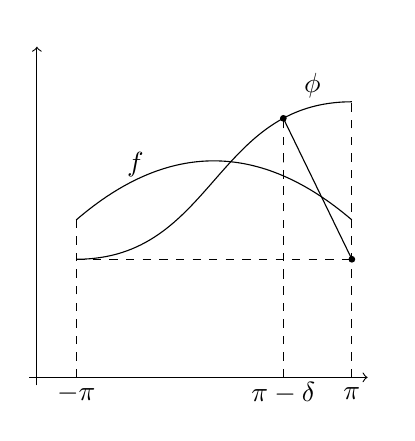
\begin{tikzpicture}
        \draw[->] (-0.1,0) -- (4.2,0) node[right] {$$};
        \draw[->] (0,-0.1) -- (0,4.2) node[above] {$$};
        \draw[scale=0.5,domain=0:4,dashed,smooth,variable=\x] plot ({1},{\x});
        \draw[scale=0.5,domain=0:7,dashed,smooth,variable=\x] plot ({8},{\x});
        \draw[scale=0.5,domain=0:6.58,dashed,smooth,variable=\x] plot ({6.26},{\x});
        \draw (0.5,2) .. controls (1.66,3) and (2.83,3) .. (4,2);
        \node at (1.25, 2.7) {$f$};
        \draw (0.5,1.5) .. controls (2.25,1.5) and (2.25,3.5) .. (4,3.5);
		\draw (3.13, 3.29) -- (4, 1.5);
		\draw[fill=black] (3.13,3.29) circle (1pt);
		\draw[dashed] (0.5, 1.5) -- (4, 1.5);
		\draw[fill=black] (4,1.5) circle (1pt);
        \node at (3.5, 3.7) {$\phi$};
		\node at (0.5, -0.2) {$-\pi$};
		\node at (4.0, -0.2) {$\pi$};
		\node at (3.13,-0.2) {$\pi - \delta$};
    \end{tikzpicture}
	\caption{КАРТИНКА}	
	\end{figure}
	В данном Случае можно просто линейно проинтерполировать 
	нужную точку и значение на границе $\delta$-окрестности (непрерывность при этом сохранится).

	\begin{gather*}
		\intl{Q} \abs{\phi - f} = \intlr{\pi - \delta}{\pi} \abs{f - \phi} \leqslant 2M \delta \leqslant \Epsilon 
	\end{gather*}
\end{proof}

Из свойств интеграла Фейера следует, что это линейный оператор, а значит, 
для него определена норма линейного оператора.

\begin{statement}
	Пусть $f \in L_p$, тогда $\normp{\sigma_n(f)} \leqslant \normp{f}$
\end{statement}

\begin{proof}
	Применим неравенство Гельдера.
	\begin{gather*}
		\normp{\sigma_n(f, x)}^p = \intl{Q} \abs{\sigma_n(f, x)} dx = 
		\intl{Q}\abs{\intl{Q}f(x + t) \Phi_n(t) dt}^pdx \leqslant
		\intl{Q} \left( \intl{Q}\abs{f(x + t)} \Phi_n(t) dt\right)^p dx = (\star) \\
		\intl{Q}\abs{f(x + t)} \Phi_n(t) dt =  
		\intl{Q} \left( \abs{f(x + t)} \Phi_n^{\frac{1}{p}}(t) \right) \Phi_n^{\frac{1}{q}}dt
		\leqslant \left( \intl{Q} \abs{f(x + t)}^p \Phi_n(t) dt\right)^{\frac{1}{p}} 
		\left( \intl{Q} \Phi_n(t)dt\right)^{\frac{1}{q}} = \\
		= \left(\text{так как} \intl{Q} \Phi_n(t)dt = 1\right) =
		\left( \intl{Q}\abs{f(x + t)}^p \Phi_n(t) dt\right)^{\frac{1}{p}} \\
		(\star) \leqslant 
		\intl{Q} \left( \intl{Q} \abs{f(x + t)}^p \Phi_n(t) dt\right) dx \stackrel{т. Фубини}{=}
		\intl{Q} \left( \intl{Q} \abs{f(x + t)}^p \Phi_n(t) dx\right) dt =
		\intl{Q} \Phi_n(t) \left( \intl{Q} \abs{f(x + t)}^p dx\right) dt = \\
		\text{(в силу $2\pi$-периодичности $f$, $\intl{Q} \abs{f(x + t)}^p dx$ - не зависит от $t$)} 
		= \normp{f}^p
	\end{gather*}

	Следовательно, $\normp{\sigma_n(f)}^p \leqslant \normp{f}^p$
\end{proof}


\begin{theorem}[Теорема Фейера в $L_p$]
	Пусть $f \in L_p$, тогда $\normp{\sigma_n(f) - f} \xrightarrow[n \rightarrow +\infty]{} 0$
\end{theorem}

\begin{proof}
	Пусть $G_n(f) = \normp{f - \sigma_n(f)} \leqslant \normp{f} + \normp{\sigma_n(f)} \leqslant 2\normp{f}$.
	\begin{enumerate}
		\item[Замечание 1]
			Пусть $g \in C$, $\abs{g(x)} \leqslant \normpp{g(x)}{C} \defeq \max\limits_{Q} \abs{g(x)}$
		\item[Замечание 2]
			$\normp{g(x)} \leqslant \left( 2\pi\right)^{\frac{1}{p}}\normpp{g(x)}{C}$
	\end{enumerate}

	По всюду плотности $C$ в $L_p$,
	$\feps > 0 \exists g_{\Epsilon} \in C : \normp{f - g_{\Epsilon}} < \Epsilon$
	\begin{enumerate}
		\item[Замечание 3]
			$G_n(f_1 + f_2) = \normp{f_2 - \sigma_n(f_2) + f_1 - \sigma_n(f_1)}\leqslant G_n(f_1) + G_n(f_2)$.
			Это называется полуаддитивность функционала.
	\end{enumerate}

	\begin{gather*}
		G_n(f) = G_n(f - g_{\Epsilon} + g_{\Epsilon}) \leqslant G_n(f - g_{\Epsilon}) + G_n(g_{\Epsilon})
		\leqslant \Epsilon + G_n(g_{\Epsilon}) \leqslant \Epsilon + \left( 2\pi \right)^{\frac{1}{p}}
		\normpp{g_{\Epsilon} - \sigma_n(g_{\Epsilon})}{C}\\
		\normpp{g_{\Epsilon} - \sigma_n(g_{\Epsilon})}{C} \xrightarrow[n \rightarrow +\infty]{} 0 
		\:\text{(в силу непрерывности $g_{\Epsilon}$)}
	\end{gather*}
	
	Следовательно, $\feps > 0\: \exists N : \forall n \geqslant N\: G_n(f) \leqslant 
	\left( 1 + \left( 2\pi\right)^{\frac{1}{p}} \right) \Epsilon$
\end{proof}

\begin{corollary}[Теорема Вейерштрасса в $L_p$]
	$\feps>0\:\forall f \in L_p\: \exists T$ - тригонометрический полином $: \normp{f - T} \leqslant \Epsilon$
\end{corollary}

\begin{proof}
	По теореме Фейера, $\normp{f - \sigma_n(f)} \xrightarrow[n \rightarrow +\infty]{} 0$.
	Значит $\exists n_0 : \normp{f - \sigma_{n_0}(f)} \leqslant \Epsilon$, теперь вспомним, что $\sigma_n(f)$ - тригонометрический полином.
\end{proof}


\subsection{Сходимость ряда Фурье в индивидуальных точках}

\begin{theorem}[Теорема Дини]
	Пусть функция $f$ и число $x$ таковы, что $\intlr{0}{\pi} \frac{\abs{\phi_x(t)}}{t}dt < +\infty$.
	
	Тогда $S_n(f, x) \xrightarrow[n \rightarrow +\infty]{} S$
\end{theorem}

\begin{proof}
	$\feps > 0$ в силу конечности интеграла, по свойствам измеримых функций:
	$\\ \exists \delta > 0: \intlr{0}{\delta} \frac{\abs{\phi_x(t)}}{t}dt < \Epsilon$
	\begin{gather*}
		\abs{S_n(f, x) - S} \leqslant \intlr{0}{\delta}\abs{\phi_x(t)}\abs{D_n(t)}dt +
		\abs{\intlr{\delta}{\pi} \phi_x(t) D_n(t) dt}
	\end{gather*}
	Как мы показывали ранее, при $t \in \left( 0 , \frac{\delta}{2}\right), 
	\sin \frac{t}{2} \geqslant \frac{t}{\pi} \Rightarrow \abs{D_n(t)} \leqslant \frac{1}{2t} $.
	Следовательно, $\abs{\phi_x(t)} \abs{D_n(t)} \leqslant \frac{1}{2} \frac{\abs{\phi_x(t)}}{t}$
	$\\ \intlr{0}{\delta} \abs{\phi_x(t)} \abs{D_n(t)} dt \leqslant \frac{\Epsilon}{2}$.
	Значит, при всех $n$ и фиксированном $\Epsilon$ 
	
	\begin{gather*}
		\abs{S_n(f, x) - S} \leqslant \frac{\Epsilon}{2} + 
		\abs{\intlr{\delta}{\pi} \phi_x(t) D_n(t)dt}
	\end{gather*}

	Так как $D_n(t) = \frac{1}{2\pi} \left( \ctg\frac{t}{2}\sin nt + \cos nt\right)$, значит

	\begin{gather*}
		\abs{\intlr{\delta}{\pi} \phi_x(t)D_n(t)dt} \leqslant 
		\frac{1}{2\pi}\abs{\intlr{\delta}{\pi} \phi_x(t) \ctg\frac{t}{2}\sin nt dt} +
		\frac{1}{2\pi}\abs{\intlr{\delta}{\pi} \phi_x(t)\cos nt dt}
	\end{gather*}

	\begin{enumerate}
		\item $\frac{1}{2\pi}\abs{\intlr{\delta}{\pi} \phi_x(t)\cos nt dt} 
			\xrightarrow[n \rightarrow +\infty]{} 0$ 
			(по лемме Римана-Лебега, так как $\phi_x(t)$ - суммируема)
		\item $\frac{1}{2\pi}\abs{\intlr{\delta}{\pi} \phi_x(t) \ctg\frac{t}{2}\sin nt dt}$
			Проверим, что $\phi_x(t)\ctg\frac{t}{2}$ - суммируема.
			
			При $\frac{t}{2} \in \left[\frac{\delta}{2}, \frac{\pi}{2} \right]$, 
			$\ctg\frac{t}{2}$ - ограничен. Следовательно, 
			$\phi_x(t)\ctg\frac{t}{2}$ - произведение суммируемой на ограниченную - суммируемо.
	\end{enumerate}
	Получаем, что начиная с $N$, $\abs{S_n(f, x) - S} < \Epsilon$
\end{proof}

\begin{corollary}[О четырех пределах]
	Пусть в точке $x$ функция $f$ - регулярна, и 
	$\alpha = \lim\limits_{t\rightarrow +0}\frac{f(x + t) - f(x + 0)}{t}$,
	$\beta = \lim\limits_{t\rightarrow +0}\frac{f(x - t) - f(x - 0)}{t}$
	(существуют обе односторонние производные).
	Тогда $S_n(f, x) \rightarrow S = \frac{f(x + 0) + f(x - 0)}{2}$
\end{corollary}
	
\begin{proof}
	Для доказательства проверим условия теоремы Дини:
	\begin{gather*}
		\abs{\phi_x(t)} \leqslant \abs{f(x + t) - f(x + 0)} + \abs{f(x - t) + f(x - 0)}\\
		\frac{\abs{\phi_x(t)}}{t} \leqslant \abs{\frac{f(x + t) - f(x + 0)}{t}} + 
		\abs{\frac{f(x - t) - f(x - 0)}{t}}\Rightarrow
		\intlr{0}{\pi} \frac{\abs{\phi_x(t)}}{t} \leqslant \pi(\alpha + \beta)
	\end{gather*}
\end{proof}


С практической точки зрения, ясно, что если дана $2\pi$-периодическая, 
кусочно-дифференцируемая функция, то в каждой точке 
ряд фурье сходится к среднему арифметическому односторонних пределов в ней.

Далее, мы будем работать с функциями из класса $\bigvee$ - функции ограниченной вариации.
\begin{statement}
	$\abs{a_n(f)}, \abs{b_n(f)} \leqslant \frac{2}{n}\veelr{-\pi}{\pi} f$
\end{statement}

\begin{proof}
	\begin{gather*}
		\abs{\frac{1}{\pi}\intl{Q}f(x)\cos nx dx} = 
		\abs{\frac{1}{\pi}\intl{Q} f(x) d\left(\sin nx \right)dx } =
		\abs{\frac{1}{\pi} \left( f(x) \sin nx \Big|_{-\pi}^{\pi} - 
		\intl{Q} \sin nx d( f(x))\right)} \leqslant \frac{2}{n}\veelr{-\pi}{\pi} f
	\end{gather*}
\end{proof}

Приведем теорему, которая формулирует условия сходимости ряда Фурье в индивидуальных точках 
(независимо от теоремы Дини).

\begin{theorem}[Теорема Дирихле]
	Пусть $f \in \bigvee$ тогда в каждой точке ее ряд Фурье 
	\begin{gather*}
		\sigma(f,x) = \frac{f(x + 0) + f(x - 0)}{2}
	\end{gather*}
\end{theorem}

\begin{proof}
	по следствию из теоремы Фейера, в силу существования, односторонних пределов, 
	ряд Фурье суммируется к $S$ по методу средних арифметических.
	Для доказательства теоремы, проверим выполнения условий Тауберовой теоремы Харди.
	Для забывчивых, ее формулировка:
	
	\begin{theorem}[Тауберова теорема Харди]
		Пусть $\sum a_n = S$ (СА). Тогда, если $\exists M - \text{const}$, такая, что
		$\forall n \in \mathbb{N} \Rightarrow 
		\sumlr{k = n + 1}{+\infty}a_k^2\leqslant \frac{M}{n}$, то ряд суммируется в обычном смысле.
	\end{theorem}

	\begin{gather*}
		A_n(f, x) = a_n \cos nx + b_n \sin nx \Rightarrow
		\abs{A_n(f, x)} \leqslant \abs{a_n(f)} + \abs{b_n(f)}
		\leqslant \frac{1}{n}4\veelr{-\pi}{\pi}f  = \frac{M}{n}\\ \Rightarrow
		\sumlr{k = n + 1}{+\infty}\abs{A_n(f, x)}^2 \leqslant 
		M^2 \sumlr{k = n + 1}{+\infty} \frac{1}{k^2} \leqslant
		M^2 \frac{1}{n}
	\end{gather*}
\end{proof}

Если брать непрерывную функцию, ограниченной вариации, то суммы Фейера равномерно сходятся к $S$.
Поэтому оценка Харди так же не зависит от $x$. 

Получим разложения в ряд Фурье функций $\text{sign}(x)$ и $\abs{x}$.



\begin{figure}[h]
\centering
\begin{tikzpicture}
    \draw[->] (-4.2,0) -- (4.2,0) node[right] {$$};
    \draw[->] (0,-4.2) -- (0,4.2) node[above] {$$};
	\draw (0, 2) -- (2, 2);
	\draw (0, -2) -- (-2, -2);
	\draw (-2, 2) -- (-4, 2);
	\draw (2, -2) -- (4, -2);
	\draw[dashed] (-2, 2) -- (-2, -2);
	\draw[dashed] (2, 2) -- (2, -2);
	\draw[dashed] (4, -2) -- (4, 0);
	\draw[dashed] (-4, 2) -- (-4, 0);
	\node at (2.1, 0.2) {$\pi$};
	\node at (-1.8, 0.2) {$-\pi$};
\end{tikzpicture}
	\caption{sign$(x)$}	
\end{figure}

Так как функция sign$(x)$ - нечетная, будем раскладывать по синусам.
\begin{gather*}
	b_n = \frac{2}{\pi}\intl{Q} \sin nx dx = 
	\frac{2}{\pi} \frac{1}{n}\cos nx \Big|_{0}^{\pi} = 
	\frac{2}{\pi n} \left(1 - (-1)^n\right) = 
	\left\{\begin{matrix}
		0, & n = 2k \\
		\frac{4}{\pi n}, & n = 2k + 1
	\end{matrix}\right.
\end{gather*}
Следовательно, 
\begin{gather*}
	f(x) = \sumlr{m = 0}{+\infty} \frac{4}{\pi (2m + 1)} \sin (2m + 1) x \\
	f\left(\frac{\pi}{2}\right) = \sumlr{m = 0}{+\infty} \frac{4(-1)^n}{\pi(2m + 1)} = 1 \Rightarrow
	\sumlr{0}{+\infty} \frac{(-1)^n}{2n + 1} = \frac{\pi}{4}
\end{gather*}


\newpage

Разложим $f(x) = \abs{x}$:

\begin{figure}[h]
\centering
\begin{tikzpicture}
    \draw[->] (-4.2,0) -- (4.2,0) node[right] {$$};
    \draw[->] (0,-4.2) -- (0,4.2) node[above] {$$};
	\draw (0, 0) -- (2, 2);
	\draw (0, 0) -- (-2, 2);
	\draw (-2, 2) -- (-4, 0);
	\draw (2, 2) -- (4, 0);
	\draw[dashed] (-2, 2) -- (-2, 0);
	\draw[dashed] (2, 2) -- (2, 0);
	\node at (2.1, 0.2) {$\pi$};
	\node at (-1.8, 0.2) {$-\pi$};
\end{tikzpicture}
	\caption{$\abs{x}$}	
\end{figure}

$f(x)$ - четная функция, значит, раскладывать будем по косинусам.
\begin{gather*}
	a_n = \frac{2}{\pi} \intlr{0}{\pi} x\cos nx dx \\
	a_0 = \frac{2}{\pi} \intlr{0}{\pi}x dx = \frac{2}{\pi} \frac{x^2}{2}\Big|_{0}^{\pi} = \pi \\
	a_n = \frac{2}{\pi}\left( \intlr{0}{\pi} x d\left(\sin nx \right)\right) = 
	-\frac{2}{\pi n} \intlr{0}{\pi} \sin nx dx = \frac{2}{\pi n^2}\cos nx \Big|_{0}^{\pi} = 
	\frac{2}{\pi n^2}\left((-1)^n - 1\right) = 
	\left\{\begin{matrix}
		0, & n = 2m \\
		-\frac{4}{\pi n^2}, & n = 2m + 1
	\end{matrix}\right.
\end{gather*}
Следовательно, $\abs{x} = \pi - \frac{4}{\pi}\sumlr{0}{+\infty}\frac{\cos ((2n + 1)x)}{(2n + 1)^2}$


\begin{gather*}
	\abs{0} = \pi - \frac{4}{\pi} \sumlr{0}{+\infty}\frac{1}{(2n + 1)^2} = 0
\end{gather*}
